%------chapter 3: works
\chapter{روش پیشنهادی} \label{chap:proposed}
در این فصل به بیان روش‌های پیشنهادی در این پژوهش برای مسئله یادگیری بدون برد می‌پردازیم. روش‌های مطرح شده در این فصل از دو رویکرد متفاوت برای حل مسئله یادگیری بدون برد استفاده می‌کنند. یک رویکرد یافتن نگاشت از فضای تصاویر به فضای توصیف دسته‌هاست که این نگاشت با استفاده از شبکه‌های ژرف مدل شده است. رویکرد دوم انجام یک خوشه‌بندی در فضای ویژگی‌های ژرف استخراج شده از تصاویر که نمونه‌های آزمون را در خوشه‌هایی تقسیم می‌کند و با یادگرفتن نگاشتی از فضای توصیف دسته‌ها به فضای ویژگی‌های ژرف تصاویر هر خوشه بر یکی از دسته‌های دیده نشده انطباق داده می‌شود. 

در ابتدای این بخش به مسئله استخراج ویژگی از تصاویر با استفاده از شبکه‌های عمیق می‌پردازیم، فضای تشکیل شده از ویژگی‌های تصاویر هنگام استفاده از این شبکه‌ها، دارای خاصیت جدایی پذیری دسته‌های مختلف از هم و تشکیل خوشه‌هایی از نمونه‌های هر دسته است؛ فرض وجود چنین خاصیت‌هایی در فضای ویژگی‌های تصاویر، اساس روش‌های ارائه شده در این فصل است.
در بخش \ref{nn} یک شبکه‌ی عصبی چندوظیفه‌ای برای پیش‌بینی ویژگی از تصاویر معرفی می‌کنیم که با در نظر گرفتن نمونه‌های آزمون در زمان آموزش می‌تواند مشکل جابجایی دامنه را کاهش دهد.
در بخش
\ref{clustering_method}
 یک تابع مطابقت نوین برای مسئله دسته‌بندی بدون برد معرفی می‌کنیم که استفاده از اطلاعات غیرنظارتی موجود در ساختار نمونه‌های دسته‌های دیده نشده را ممکن می‌سازد. این تابع مطابقت از یک خوشه‌بندی روی نمونه‌های آزمون بهره می‌برد که با توجه به استخراج ویژگی‌ها با استفاده از شبکه‌های عصبی عمیق و جداسازی مناسب در فضای این ویژگی‌ها، از دقت مناسبی برخوردار است. این تابع مطابقت به نمونه‌هایی که در یک خوشه قرار دارند برچسب یکسانی نسبت می‌دهد. با توجه به استفاده از خوشه‌بندی در این تابع مطابقت، یک روش خوشه‌بندی نیمه‌نظارتی که منطبق بر فرضیات مسئله یادگیری بدون برد است ارائه می‌گردد و سپس یک روش دسته‌بندی با استفاده از تابع مطابقت و خوشه‌بندی ارائه شده و یادگیری نگاشتی خطی از توصیف دسته‌ها به فضای تصاویر، تدوین می‌گردد. هرچند که عملکرد این روش ارائه شده برتر از روش‌های پیشگام موجود است ولی محدودیت‌هایی نیز دارد که ناشی از جدا بودن مرحله خوشه‌بندی و نگاشت به فضای مشترک است؛ برای رفع این محدودیت‌ها روش دیگری معرفی می‌شود که خوشه‌بندی و یادگیری نگاشت در آن به صورت توام انجام می‌شود. این یادگیری توام باعث بهبود دقت دسته‌بندی نسبت به روش پیشنهادی قبلی می‌شود.

نمادگذاری مورد استفاده در این فصل سازگار با نمادگذاری معرفی شده در بخش ۲ است که در جدول \ref{tab:notation} برای مراجعه سریع خلاصه شده است.
\begin{center}
\begin{table}[ht]
\centering
\caption{معرفی نمادهای مورد استفاده}
\vspace{2mm}
\label{tab:notation}
\begin{tabular}{|c|r|}
\hline
 نماد &  شرح \\
\hline
  $\mathcal{S}(\mathcal{U})$ & \rl{مجموعه دسته‌های دیده‌شده (دیده‌نشده) }     \\\hline
  $n_s (n_u) $ & \rl{تعداد دسته‌های دیده‌شده (دیده‌نشده) }   \\\hline
  $N_s (N_u) $ & \rl{تعداد نمونه‌های آموزش (آزمون) }   \\\hline
  $X_s (X_u) $ & \rl{ماتریس نمونه‌های آموزش (آزمون) }   \\\hline
  $Y_s (Y_u) $ & \rl{برچسب‌های نمونه‌های آموزش (آزمون) }   \\\hline
  $C_s (C_u) $ & \rl{ماتریس توصیف‌های دسته‌های دیده‌شده (دیده‌نشده) }   \\\hline
  $\mathbf{x_i}  \in \mathbb{R}^d$ & \rl{ بردار ویژگی‌های تصویر $-i$م}   \\\hline
 $ \mathbf{c_y}  \in \mathbb{R}^a$ & \rl{بردار توصیف دسته‌ی $y$}   \\\hline
\hline
 $X_{(i)}$ & \rl{سطر $-i$م ماتریس $X$} \\ \hline
 $\normf{X}$ & \rl{نرم فروبنیوس ماتریس $X$} \\ \hline
 $diag(\mathbf{x})$ & \rl{یک ماتریس قطری که بردار $\mathbf{x}$ روی قطر اصلی آن قرار داده شده} \\ \hline
 $\mathbf{1}$ & \rl{یک بردار که تمام عناصر آن برابر یک است} \\ \hline
 $\mathbf{1}_k$ & \rl{یک بردار که درایه‌ی $-k$م آن یک و سایر عناصرش صفر است } \\ \hline
\end{tabular}
\end{table}
\end{center}

\section{استخراج ویژگی با شبکه‌های عصبی عمیق}\label{cnns}
عمل‌کرد مناسب روش‌های بینایی ماشین از جمله روش‌هایی دسته‌بندی بدون برد تصاویر  وابستگی زیادی به نمایش بدست آمده از تصاویر دارد. در سال‌های اخیر استفاده از شبکه‌های عصبی پیچشی ژرف کاراترین روش برای استخراج ویژگی از تصاویر بوده است \cite{Oquab2014}. این روش که در آن نحوه‌ی استخراج ویژگی با استفاده از تعداد زیادی داده‌ی برچسب‌دار
\textit{یاد گرفته می‌شود،}
جایگزین روش‌های قبلی مانند SIFT و HOG شده است که در آن‌ها، نحوه‌ی استخراج ویژگی توسط یک خبره تعیین شده و همواره ثابت است.

معماری شبکه‌های عصبی ژرف پیچشی مبتنی بر خاصیت \gls{stationary} بودن تصاویر است، این خاصیت به این معناست که خواص آماری نواحی مختلف تصاویر با یکدیگر یکسان هستند. در نتیجه‌ی وجود این خاصیت \gls{filter} مورد برای استخراج \gls{localfeat} از تصویر در تمام مکان‌های تصویر یکسان در نظر گرفته می‌شود. چنین نگاشتی با عمل پیچش قابل مدل‌سازی است. فرض کنید که $v$ یک تصویر $M\times N$ باشد و $W$ یک صافی خطی، آن‌گاه یک لایه‌ی پیچشی از یک شبکه عصبی به صورت زیر تعریف می‌شود:
\begin{align}
h_1^{(k)} &= g(W^k \ast v + b^k) \label{eq:conv_layer}\\
(W \ast x)_{m,n} &= \sum_{i=-\infty}^{\infty} \sum_{j=-\infty}^{\infty} W_{i,j} x_{m -i, n-j}.
\end{align}
در این رابطه $h^{(1)}$ مقادیر لایه نهان اول شبکه را نشان می‌دهد و $b$ جمله‌‌ی بایاس است، $g$ یک  \gls{ActivationFunction} مانند $tanh$ است. در این حالت فیلتر $W$ که عموما اندازه بسیار کمتری نسبت به تصویر دارد (برای مثال $3 \times 3$ یا
$ 7 \times 7$)
بر تصویر اعمال می‌شود تا ویژگی‌هایی از تصویر استخراج کند. این مدل‌سازی مشابه روش‌های قدیمی‌تری است که مثلا برای تشخیص لبه و گوشه استفاده می‌شوند \cite{harris1988}. مهم‌ترین تفاوت شبکه‌های عصبی و آن روش‌ها در این است که مقادیر فیلتر $W$ یادگرفته می‌شوند و از پیش توسط خبره معین نشده‌اند. همچنین در این شبکه‌ها در هر لایه عموما از چندین صافی استفاده می‌شود و چند  تعداد کم پارامترهای فیلتر و استقلال آن از اندازه تصویر ورودی، باعث شده تعداد پارامتر‌های موجود در یک لایه‌ی پیچشی بسیار کمتر از یک \gls{fully-connected-layer} باشد و در نتیجه امکان افزایش عمق شبکه بیشتر باشد. در نتیجه در شبکه‌های عصبی معمولا از چندین لایه‌ی پیچشی استفاده می‌شود. 
\begin{figure}[!t]
\centering
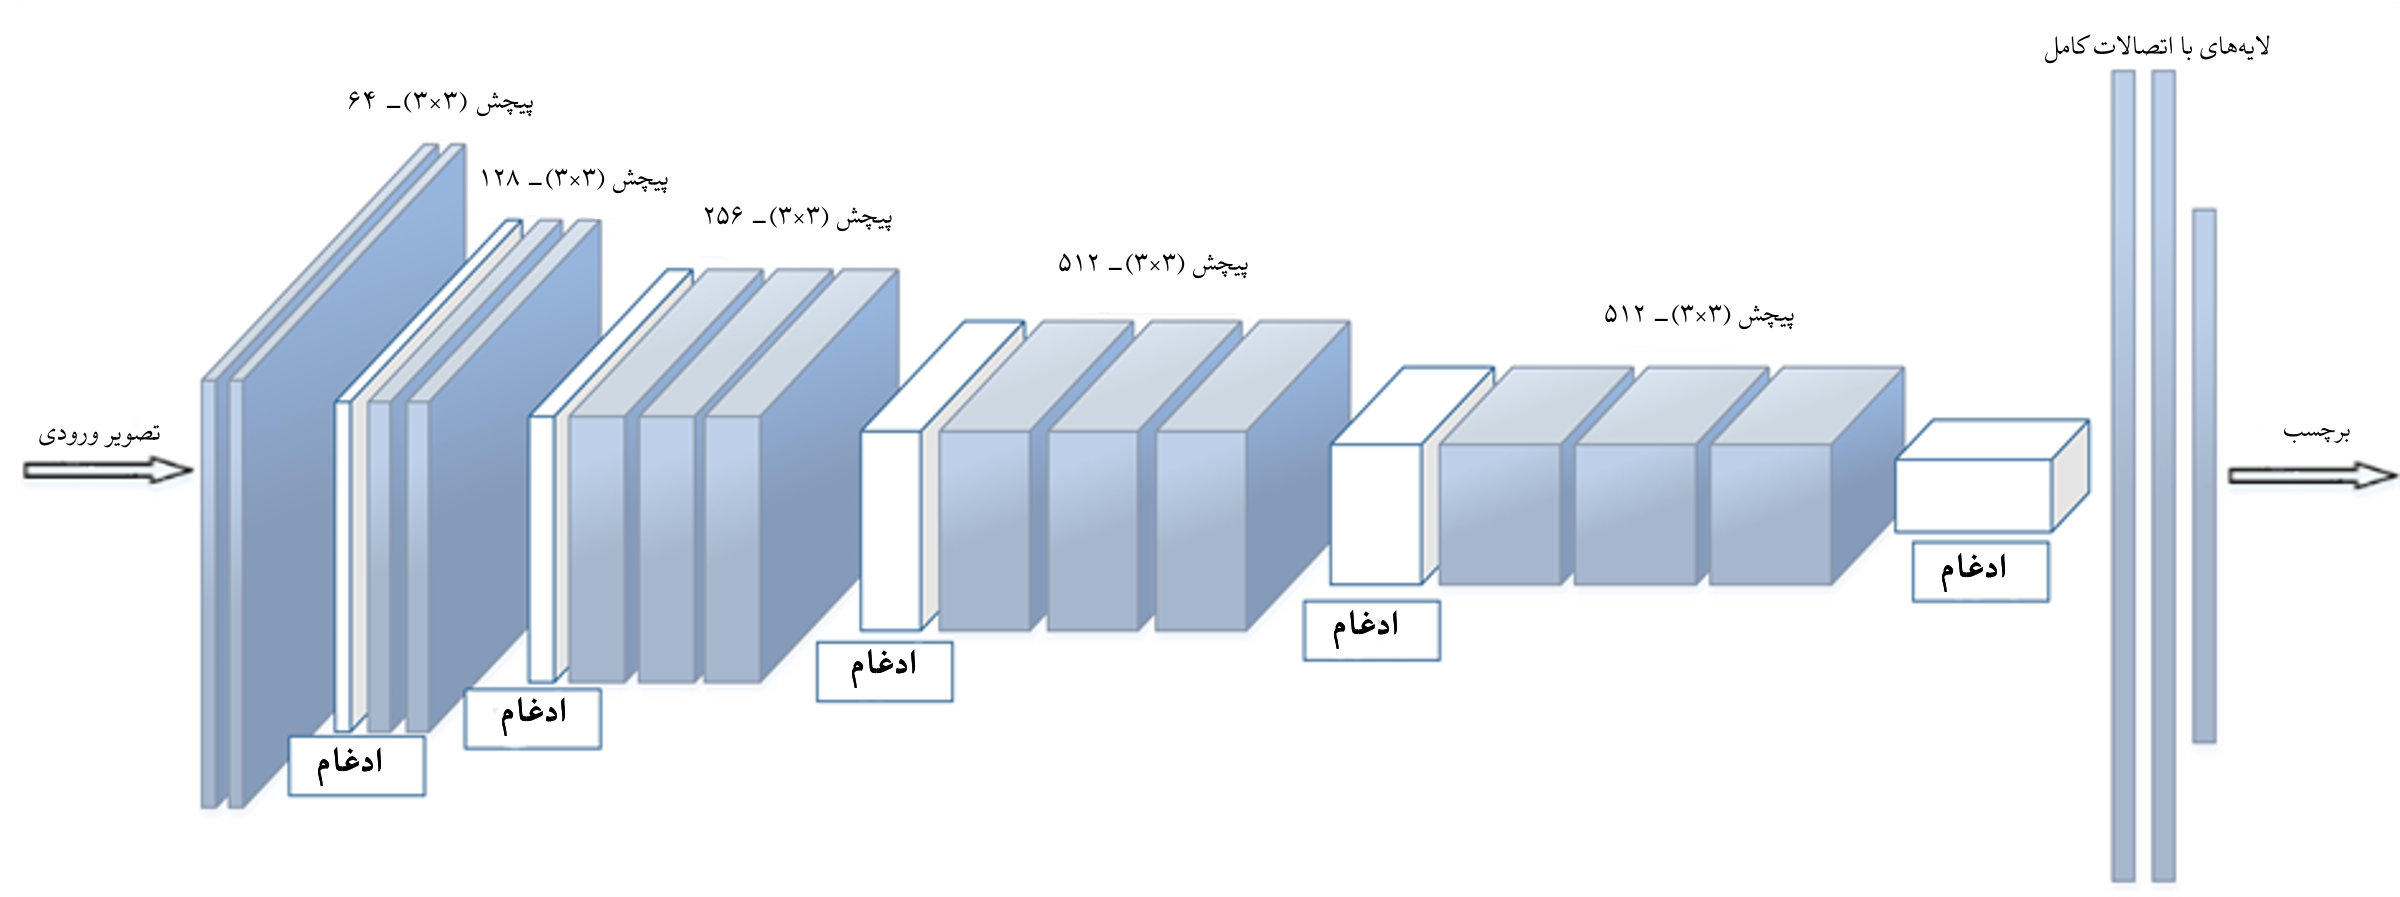
\includegraphics[width=1.1\linewidth]{images/vgg}
\caption[ساختار شبکه استخراج ویژگی]{
ساختار شبکه vgg که در آن لایه‌های سفید مراحل ادغام که اینجا انتخاب بیشینه در پنجره‌های $2 \times 2$ است را نشان می‌دهند.
لایه‌های پیچشی با مکعب‌های آبی مشخص شده‌اند که عرض آن‌ها متناسب با تعداد کانال‌های موجود در آن لایه است \cite{el2016face}.
}
\label{fig:vgg}
\end{figure}
معماری مورد استفاده در روش‌های این فصل برای استخراج ویژگی، مبتنی بر معماری ۱۹ لایه شبکه \lr{vgg} \cite{vgg} است (شکل \ref{fig:vgg}). در این شبکه از ۱۶ لایه‌ی پیچشی استفاده شده است. ساختار هر لایه به این صورت است که تعدادی کانال از ویژگی‌ها (در لایه‌ی اول  خود تصویر) به عنوان ورودی وارد لایه می‌شوند و با استفاده از تعدادی صافی با اندازه $3 \times 3$ به ویژگی‌های خروجی تبدیل می‌شوند. تعداد کانال‌های ورودی در لایه‌ی اول سه کانال رنگی \lr{RGB} است و در لایه‌های بعدی تعداد صافی‌ها به گونه‌ای تعیین شده که تعداد کانال‌های ویژگی‌ها برابر: ۶۴ در لایه‌ی اول و دوم، ۱۲۸ در لایه‌ سوم و چهارم، ۲۵۶ در لایه پنجم تا هشتم و ۵۱۲ در لایه نهم تا شانزدهم است. \gls{ActivationFunction} مورد استفاده در لایه‌های پیچشی تابع \gls{ReLU} است که ضابطه آن به این صورت است:
\begin{equation}
ReLU(\mathbf{x}) = max(\mathbf{0,x}).
\end{equation}
 برای کاهش اندازه ماتریس ویژگی‌ها، میان برخی لایه‌های پیچشی از یک تابع \gls{pooling} استفاده می‌شود. تابع \gls{pooling} مورد استفاده در این شبکه تابع \gls{pooling} بیشینه است یعنی در ماتریس ویژگی‌ حاصل یک پنجره‌ی $2 \times 2$ حرکت داده می‌شود و تنها بزرگترین مقدار میان چهار مقداری پنجره بر آن‌ها منطبق شده به خروجی منتقل می‌شود. بعد از ۱۶ لایه پیچشی سه \gls{fully-connected-layer} وجود دارد. ما برای استخراج ویژگی از خروجی لایه‌ی هدفهم یعنی نخستین  \gls{fully-connected-layer} استفاده می‌کنیم و دو لایه‌ی نهایی کنار گذاشته می‌شوند. ورودی این لایه به این صورت به دست می‌آید که تمام ماتریس‌های ویژگی لایه‌ی شانزدهم به صورت بردارهای یک بعدی در آمده و در کنار هم قرار می‌گیرند، سپس به صورت یک برادر $-25088$ بعدی وارد لایه‌ی هفدهم شده و در این لایه با استفاده از یک نگاشت خطی و \gls{ActivationFunction}   \gls{ReLU} به بردارهای ویژگی $-4096$بعدی تبدیل می‌شود. در شبکه اصلی این خروجی این لایه به یک لایه‌ی مشابه خود و سپس در نهایت با یک لایه \gls{fully-connected-layer} که خروجی آن به اندازه تعداد دسته‌هاست با  \gls{ActivationFunction} 
 \lr{softmax}
 به پیش‌بینی برچسب تبدیل می‌شود. 
 
\section{یک شبکه‌عصبی چندوظیفه‌ای}\label{nn}
\begin{figure}[!t]
\centering
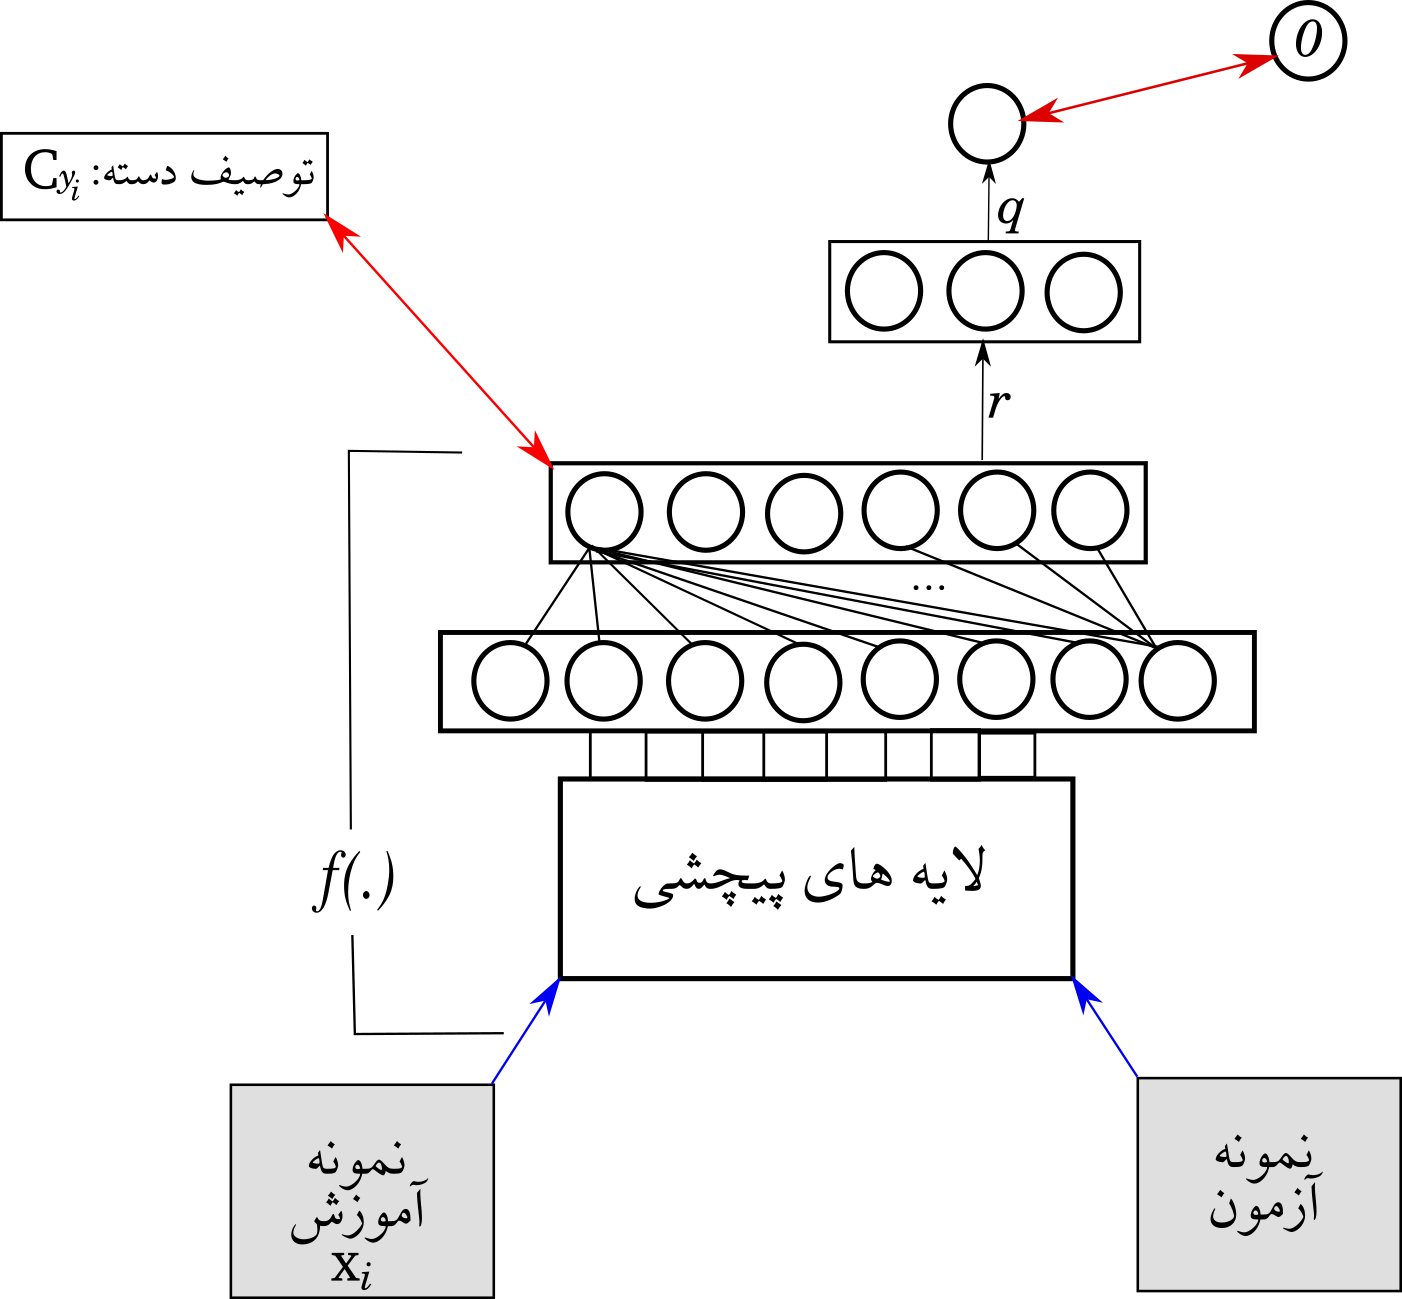
\includegraphics[width=0.85\linewidth]{images/net}
\caption[شبکه‌ی چندوظیفه‌ای پیشنهادی]{
ساختار شبکه چند وظیفه‌ای پیشنهادی. فلش‌های آبی رنگ ورودی‌های شبکه را نشان می‌دهند و فلش‌های قرمز رنگ مقایسه خروجی شبکه با خروجی مورد انتظار را. خطوط سیاه‌رنگ اتصالات شبکه‌ را نشان می‌دهند. زیر شبکه‌ی برگرفته شده از شبکه vgg و یک لایه‌ی با اتصالات چگال اضافه شده بین دو دو ورودی مشترک هستند. لایه‌های $r$ و $q$ مخصوص نمونه‌های آزمون هستند. خروجی لایه‌ی $q$ همواره با مقدار صفر مقایسه می‌شود.
}
\label{fig:nn2}
\end{figure}

یادگیری نگاشت‌ها با استفاده از داده‌های دسته‌های دیده‌شده، همان‌طور که در بخش \ref{lr:semi} اشاره شد، دچار مشکل جابجایی دامنه است و  روی داده‌های دسته‌های دیده‌نشده به خوبی قابل تعمیم نیست. یک راه حل برای مقابله با این مشکل این است که در حین یادگیری نگاشت اجبار شود که حاصل نگاشت یک نمونه‌ی آزمون به نوعی نزدیک به نگاشت توصیف دسته‌های آزمون باشد. همان ‌طور که در بخش
\ref{lr:semi}
بیان شد، چنین راه‌حلی در
\cite{Kodirov2015}
استفاده شده است. معیار نزدیکی نگاشت‌ها در آن روش یک امتیاز پیشین از شباهت هر نمونه‌ی آزمون با دسته‌های دیده نشده است که  توسط یک روش دیگر استخراج شده می‌شود. یعنی ابتدا یک روش دسته‌بندی 
احتمالی  که در آن پژوهش روش \lr{IAP} \cite{lampert09} برای این کار انتخاب شده بود، به صورت مستقل روی مجموعه دادگان اجرا شده و احتمال‌هایی که برای انتساب هر نمونه به دسته‌های آزمون از آن روش بدست می‌آید بعنوان وزن‌های شباهت در نظر گرفته می‌شود و فاصله هر توصیف پیش‌بینی شده برای هر نمونه با توصیف دسته‌های آزمون متناسب با این وزن‌های شباهت جریمه می‌شود.
 ما در این بخش یک روش مبتنی بر شبکه‌های عصبی عمیق معرفی می‌کنیم که در آن نگاشتی غیرخطی و چندلایه از تصاویر به بردارهای ویژگی یادگرفته می‌شود. معیار یادگیری این نگاشت، پیش‌بینی صحیح ویژگی برای نمونه‌های آموزش (که بردار ویژگی صحیح برای آن‌ها مشخص است) و هم‌چنین نزدیک بودن حاصل نگاشت هر نمونه‌ی آزمون به توصیف یکی از دسته‌های دیده نشده است. برای مدل کردن این نگاشت، از یک شبکه‌ی عصبی استفاده شده است. اگر نگاشت مدل شده با شبکه عصبی را با $f$ نشان دهیم، تابع هزینه‌ی مورد استفاده برای آموزش شبکه به صورت زیر تعریف می‌شود:
\begin{equation}
\label{eq:nn_loss}
\min_{f}
\frac{1}{N_s} \sum_{n=1}^{N_s} loss(f(\mathbf{x_i), c_{y_i}}) +
\frac{\beta}{N_u} \sum_{i=N_s}^{N_s+N_u} \Big ( \min_{j=n_s,\ldots,n_s + n_u} \normtwo{f(\mathbf{x_i) - c_j}} \Big ),
\end{equation}
که $\beta$ یک فراپارامتر است.
جمله‌ی اول، جمله‌ی مربوط به خطایی پیش‌بینی صفت‌هاست تفاوت میان صفات پیش‌بینی شده توسط شبکه و صفات صحیح را برای نمونه‌های آموزش جریمه می‌کند. 
 جمله‌ی دوم برای رفع مشکل جابجایی دامنه طراحی شده است و تحمیل می‌کند که حاصل نگاشت یک نمونه‌ی آزمون حتما نزدیک توصیف یکی از دسته‌های دیده‌نشده باشد، این دسته‌ی دیده نشده، دسته‌ای در نظر گرفته شده است که توصیف آن با نگاشت کمترین فاصله را دارد. این قسمت از رابطه فوق را می‌توان به صورت شهودی این گونه توضیح داد که در غیاب جمله‌ی دوم برای هر نمونه یک بردار توصیف پیش‌بینی می‌شد و سپس نزدیک‌ترین بردار توصیف از میان توصیف دسته‌های آزمون به عنوان توصیف صحیح در نظر گرفته شده و برچسب بر اساس آن پیش‌بینی می‌شد. حال جمله‌ی دوم رابطه \eqref{eq:nn_loss} جریمه‌ای به میزان فاصله‌ی توصیف پیش‌بینی شده برای هر نمونه با بردار توصیف همان دسته‌ای که به آن نزدیک‌تر است، در نظر می‌گیرد. حال اگر این فرض صحیح باشد که 
 حاصل نگاشت در اکثر موارد به توصیف صحیح نزدیکتر است، یا به عبارتی این که در اکثر مواقع استفاده از دسته‌بند نزدیکترین همسایه روی نگاشتی که تنها با جمله‌ی اول آموزش دیده، دقتی بیش از ۵۰٪ دارد، وجود چنین جمله‌ای باعث می‌شود که مواردی که قبلا درست تشخیص داده می‌شدند حالا با دقت بیشتر (فاصله کمتر از بردار توصیف دسته‌ی مورد نظر) باز هم درست پیش‌بینی شوند. با توجه به افزایش دقت نگاشت روی این نمونه‌ها، انتظار می‌رود برای برخی نمونه‌هایی که در حالت قبل پیش‌بینی نادرست به آن‌ها تعلق می‌گرفت نیز با این نگاشت بهبود یافته، پیش‌بینی صحیح برای آن‌ها صورت بگیرد.
 
 تابع $loss(\cdot, \cdot)$ در معادله \eqref{eq:nn_loss} در مجموعه دادگانی که صفات دودویی هستند تابع \gls{crossentropy} متقاطع در نظر گرفته شده است یعنی:
 \begin{equation}
 loss(y,z) = z \log(1-y) + (1-z) \log(y). 
 \end{equation}
 برای مجموعه دادگانی که مقادیر بردارهای توصیف در آن‌ها مقادیر دلخواه حقیقی است تابع خطای مربع اختلاف در نظر گرفته شده است:
 \begin{equation}
 loss(y,z) = \normtwo{y-z}.
 \end{equation}
 \subsection{بهینه‌سازی }\label{opt_nn}
 
 تابع کمینه به کاربرده شده در جمله‌دوم معادله
\eqref{eq:nn_loss}
در برخی نقاط مشتق‌پذیر نیست، اما با توجه به اینکه اندازه‌ی این نقاط صفر است تابع تقریبا همه‌جا مشتق‌پذیر است و آموزش شبکه با استفاده از \gls{backprop}
 مقدار گرادیان ممکن خواهد بود. به صورت دقیق‌تر، بهینه‌سازی رابطه \eqref{eq:nn_loss} عملیات محاسبه‌ی مقدار کمینه را داخل شبکه تعبیه می‌کنیم (شکل \ref{fig:nn2})؛ به این صورت که لایه‌های جدید $q$ و$r$ برای نمونه‌های دیده نشده اضافه می‌شود که:
\begin{align}
\label{eq:min_layer}
(q(\mathbf{v}))_j &=  \normtwo{f(\mathbf{v) - c_j}}, \\
r(\mathbf{z}) &= \min_{j=1\ldots n_u} (\mathbf{z})_j.
\end{align}
در رابطه \eqref{eq:min_layer}، لایه‌ی $q$ یک بردار توصیف پیش‌بینی شده را به در ورودی دریافت کرده است و خروجی آن برداری است که تعداد ابعادش برابر تعداد دسته‌های دیده‌نشده است و مقدار هر بعد آن برابر فاصله‌ی بردار $v$ با بردار توصیف (امضای) یک دسته‌ی دیده‌نشده. سپس خروجی این لایه به لایه‌ی $r$ وارد می‌شود و در این لایه کوچکترین مقدار این بردار انتخاب می‌شود. نتیجتاً ترکیب این دولایه کمینه‌ی فاصله‌ی $v$ با امضاهای دسته‌های دیده‌نشده را تولید خواهد کرد که برابر جمله‌ی دوم در رابطه \eqref{eq:nn_loss} خواهد بود.

در هنگام آموزش با پس‌انتشار، مشق تابع هزینه‌ی $l$ نسبت به هر ورودی مثل $z$ در لایه‌ی $r$ با ضابطه‌ی زیر محاسبه می‌شود:
\begin{equation}
\label{eq:grad_min}
\frac{\partial l}{\partial z} = \sum_j \mathds{1}[(z)_j=\min(z)] \cdot \frac{\partial l}{(z)_j}.
\end{equation}

پس از آموزش شبکه، در فاز آزمون لایه‌های $q$ و $r$ حذف شده و بردار توصیف برای تصاویر آزمون با استفاده از شبکه پیش‌بینی می‌شود، در نهایت دسته‌بندی با استفاده از دسته‌بند نزدیک‌ترین همسایه روی نمونه‌های آزمون انجام خواهد شد. برای اندازه‌گیری میزان شباهت بردارهای صفات در این دسته‌بند از فاصله منهتنی استفاده کرده‌ایم:
\begin{equation}
y^{\star}_n = \mathbf{1}_{\argmin_{j} \norm{f(\mathbf{x_n - c_j})}_1} .
\end{equation}
مراحل آموزش شبکه در الگوریتم \ref{alg:nn} آورده شده است.
\شروع{program}[t!]
	\begin{enumerate}[label={\arabic*},itemsep=.1em, parsep=.1em]
\فقره {\bf ورودی:} تصاویر و توصیف‌های آموزش و آزمون و برچسب‌های نمونه‌های آموزش.
\فقره {\bf خروجی:} برچسب‌های پیش‌بینی شده برای نمونه‌های آزمون.
\فقره پیش آموزش شبکه تنها با نمونه‌های آموزش و مقایسه خروجی با توصیف صحیح.
\فقره آموزش کامل شبکه با داده‌های آموزش و آزمون.
\فقره حذف لایه‌های $r$ و $q$.
\فقره خروجی شبکه را به ازای $X_u$ در $P_u$ بریز.
\فقره دسته‌بند نزدیک‌ترین همسایه $NN$ را با بردارهای توصیف دسته‌های آزمون بساز
\فقره عناصر $P_u$ را با استفاده از $NN$ دسته‌بندی کن.
\فقره حاصل مرحله قبل را به عنوان پیش‌بینی نهایی برگردان.
\end{enumerate}
\caption{الگوریتم آموزش و آزمون شبکه عصبی پیشنهادی}
\label{alg:nn}
\پایان{program}
\subsection{معماری شبکه}\label{net_architechture}
ما از قسمتی از شبکه‌ی ۱۹ لایه‌ی \lr{vgg} \cite{vgg} که شامل ۱۶ لایه‌ی پیچشی ابتدا و لایه‌‌‌اول با اتصالات چگال به عنوان یک زیر شبکه در ورودی شبکه خود استفاده می‌کنیم. همان‌طور که در بخش 
\ref{cnns}
شرح داده شد،
 با این زیر شبکه تصاویر ورودی به بردارهای $-4096$بعدی نگاشته می‌شنود. سپس یک لایه‌ی با اتصالات چگال قرار دارد که این حاصل را به بردارهای توصیف دسته‌ها می‌نگارد. برای نمونه‌های آموزش، خروجی این لایه با بردار توصیف صحیح مقایسه می‌شود. برای نمونه‌های آزمون خروجی این لایه به  لایه‌های  $q$ و$r$ متصل می‌شود و مقدار خروجی $r$ با مقدار مطلوبش که صفر است مقایسه خواهد شد.

\gls{ActivationFunction} در همه‌ی لایه‌ها تابع \gls{ReLU} است؛ با این استثنا که برای مجموعه‌ دادگانی که مقادیر بردار توصف دودویی هستند، در لایه‌ی آخر از تابع سیگموید با ضابطه 
\begin{equation}
\sigma(x) = \frac{1}{1 + e^{-x}},
\end{equation}
بعنوان \gls{ActivationFunction} استفاده شده است تا مقادیر در بازه‌ی $[0,1]$ نگاشته شوند.

\subsection{یک مدل پایه برای مقایسه}\label{nn_basic}
برای روشن شدن تاثیر استفاده از اطلاعات بدون نظارت نمونه‌های آزمون در یادگیری بهتر نگاشت، مدل ارائه شده را با یک مدل ساده برای پیش‌بینی ویژگی مقایسه می‌کنیم. در این مدل ساده تنها  از
\glspl{fully-connected-layer}
بعد از استخراج ویژگی با لایه‌های پیچشی، برای پیش‌بینی ویژگی استفاده می‌کنیم. ساختار این مدل در تصویر \ref{fig:nn_basic} نمایش داده شده است. در این شبکه از یک یا چند 
\gls{fully-connected-layer}
بعد از لایه‌های پیچشی استفاده می‌شود. مشابه حالت قبل \gls{ActivationFunction} برای مجموعه دادگانی که مقادیر توصیف دسته‌هایشان دودویی است تابع سیگموید، و برای مجموعه دادگانی که مقادیر بردارهای توصیف در آن‌ها مقادیر دلخواه حقیقی است تابع \gls{ReLU} استفاده شده است. 
ابعاد  \gls{fully-connected-layer} پایانی الزاما برابر تعداد ابعاد بردارهای توصیف است و برای سایر   \gls{fully-connected-layer} نیز همین تعداد ابعاد انتخاب شده است. 
مقایسه نتایج دقت دسته‌بندی بین مدل قبلی و این مدل در بخش \ref{exp:nn} نشان‌دهنده‌ی تاثیر مثبت استفاده از اطلاعات بدون نظارت موجود در نمونه‌های آزمون است که باعث بهبود حداقل ۱۰ درصدی دقت دسته‌بندی شده است.
\begin{figure}[!ht]
\centering
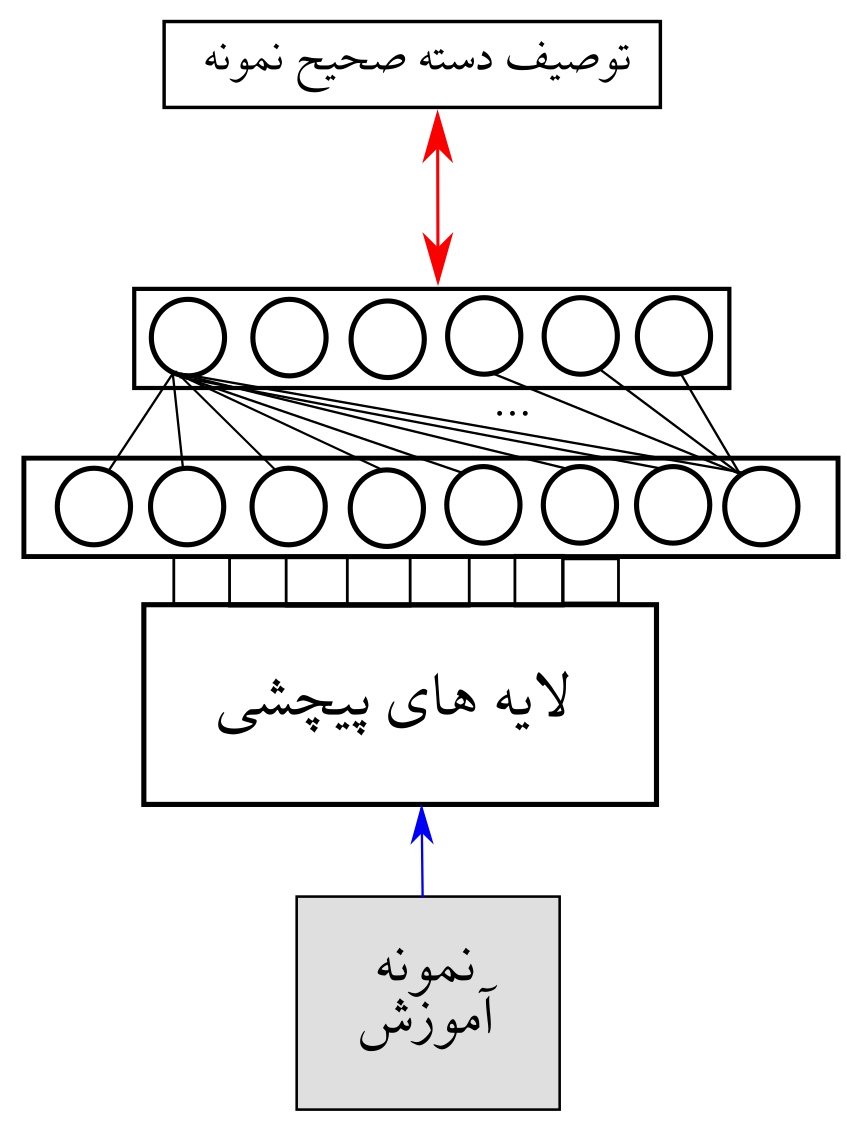
\includegraphics[width=0.4\linewidth]{images/basic_net}
\caption[شبکه‌ی پایه برای پیش‌بینی ویژگی]{
ساختار شبکه پایه. فلش آبی رنگ ورودی‌های شبکه را نشان می‌دهند و فلش‌های قرمز رنگ مقایسه خروجی شبکه با خروجی مورد انتظار را.}
\label{fig:nn_basic}
\end{figure}
\section{ تابع مطابقت مبتنی بر خوشه‌بندی }\label{compatibility_funcion}
در اکثر روش‌های پیشین که در فصل \ref{chap:lr} مرور شد، تابع مطابقت میان تصاویر و توصیف‌ها برای اختصاص برچسب به داده‌های آزمون بر اساس فاصله کمینه یا ضرب داخلی بیشینه در یک فضای مشترک محاسبه می‌شد. استثناهای این موضوع، استفاده از روش انتشار برچسب در \cite{Fu2014} و \cite{Kodirov2015} و هم‌چنین پیش‌بینی مستقیم برچسب‌ها در
\cite{li15max}
و
\cite{semi15}
هستند.

\begin{figure}[!t]
\centering
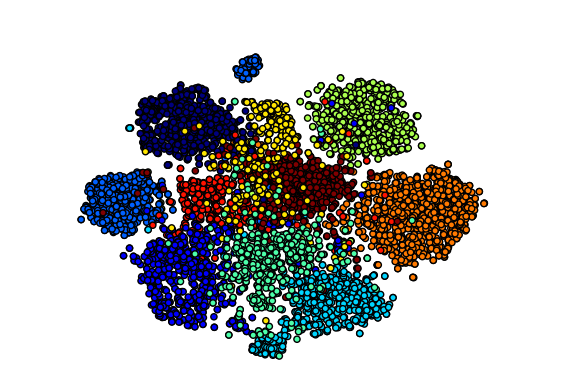
\includegraphics[width=0.85\linewidth]{images/awa_clusters}
\caption[نمایش دسته‌های آزمون مجموعه دادگان AwA ]{
نمایش دوبعدی بوسیله \lr{t-SNE} برای ده دسته‌ی آزمون از مجموعه دادگان AwA با ده رنگ متفاوت نشان داده شده است. درستی فرض قابل خوشه‌بندی در تصویر مشخص است، یعنی ویژگی‌های استخراج شده با استفاده از شبکه‌های عمیق توانایی ایجاد تمایز بالا میان دسته‌ها را دارا هستند.
}
\label{fig:awa_clusters}
\end{figure}

در این بخش ما یک تابع مطابقت جدید بر اساس یک خوشه‌بندی روی داده‌های دسته‌های دیده نشده، تعریف می‌کنیم. اگر فضای نمایش تصاویر دارای این خاصیت باشد که دسته‌های مختلف به صورت خوشه‌های مجزا باشند، استفاده از خوشه‌بندی برای دسته‌بندی برای انتساب برچسب از نظر شهودی توجیه‌پذیر است.
با توجه به نمایش غنی بوجود آمده برای تصاویر توسط شبکه‌های عمیق این فرض در بسیاری از موارد برقرار است. برای نمونه، نمایش \lr{t-SNE} نمونه‌های آزمون مجموعه داده‌های AwA در تصویر
\ref{fig:awa_clusters}
نشان داده شده است و برقراری فرض قابل خوشه‌بندی بودن در آن قابل مشاهده است. این ادعا با استفاده از آزمایش در بخش
\ref{exp:cluster}
اثبات خواهد شد. روش‌های پیشنهادی ما در این فصل بر اساس این ساختار و استفاده از وجود چنین خاصیتی در فضای تصاویر است.
%\section{معرفی یک تابع مطابقت}\label{copatibility_function}

یک راه استفاده از چنین خاصیتی در فضای تصاویر، معرفی یک تابع مطابقت است که علاوه بر شباهت نگاشت‌یافته‌ی نمونه‌ها و توصیف‌ها به سایر نمونه‌های در همسایگی هر نمونه نیز وابسته باشد. بدین منظور ما یک تابع مطابقت جدید پیشنهاد می‌دهیم که در آن برچسب تعلق گرفته به هر نمونه به نمونه‌هایی که با آن‌ها در یک خوشه قرار گرفته است وابسته است. به این منظور ابتدا باید یک خوشه‌بندی روی نمونه‌ها انجام شود سپس با استفاده از یک معیار (که یک نمونه از آن را در بخش \ref{simple_method} معرفی می‌کنیم) میزان شباهت خوشه به توصیف تعیین می‌شود. این در مقابل حالتی است که تابع مطابقت، میزان شباهت هر نمونه را به طور جداگانه با توصیف دسته‌ها محاسبه می‌کرد.  در این حالت هر خوشه باید یک برچسب دریافت کند و برچسب اختصاص یافته به هر خوشه، توسط تمام اعضای آن به ارث برده می‌شود. این تابع مطابقت تا کنون در روش‌های موجود برای یادگیری بدون برد استفاده نشده بوده است. نسخه‌های متفاوتی از این تابع مطابقت بر حسب چگونگی تعیین برچسب هر خوشه قابل ارائه است که ما در اینجا دو مورد از آن‌ها را بیان می‌کنیم. 
یک نحوه برای انتساب خوشه‌ها به دسته‌های دیده نشده استفاده از رای اکثریت است، در این حالت بایست ابتدا یک پیش‌بینی برای همه نمونه‌های آزمون صورت بگیرد (برای مثال با استفاده از روش معرفی شده در بخش \ref{nn})، فرض کنید که این برچسب‌گذاری را با 
$z_n$
برای
 $N_s < n \leq N_s + N_u$
نشان دهیم. هم‌چنین یک خوشه‌بندی روی داده‌ها انجام شده که آن را با 
$r_n$ برای 
$N_s < n \leq N_s + N_u$
نشان می‌دهیم. حال   $\ell(k)$ که برچسب خوشه‌ی $-k$م است از رابطه زیر تعیین خواهد شد:
\begin{equation}
\ell(k) = \argmax_{n_s < i \leq n_s + n_u} \, \Big [ \sum_{m=N_s+1}^{N_s+N_u} \mathds{1}(r_n = k) \times \mathds{1}(z_n = i) \Big ].
\end{equation}
در این حالت،
 این تابع مطابقت قابل اضافه شدن به روش‌های دیگر نیز می‌باشد. به این صورت که پیش‌بینی‌های انجام شده در آن روش را در نظر گرفته و با استفاده از آن‌ها در هر خوشه رای‌گیری انجام دهیم تا برچسبی که کل خوشه دریافت می‌کند تعیین شود. آزمایش‌ها نشان می‌دهند که  اضافه شدن این تابع مطابقت عمل‌کرد شبکه عصبی چندوظیفه‌ای پیشنهادی را بهبود می‌دهد.
 
 یک نسخه‌ی دیگر از این تابع مطابقت که در روش ارائه شده در بخش \ref{simple_method} مورد استفاده قرار می‌گیرد مربوط به حالتی است که نگاشتی از فضای توصیف دسته‌ها به فضای تصاویر وجود داشته باشد. فرض کنید که چنین نگاشتی یادگرفته شده و با $\theta$ نشان داده شود. هم‌چنین نگاشت 
 $\phi(x)$
  نگاشت تبدیل تصاویر به ویژگی‌های ژرف است. مانند حالت قبل یک خوشه‌بندی $r_n$ روی نمونه‌های آزمون صورت گرفته و
   $\boldsymbol{\mu_k} $
    مرکز خوشه $-k$م را نشان می‌دهد. در نتیجه داریم:
 \begin{equation}
 r_n = \argmin_{k} \normtwo{\phi(\mathbf{x_n}) - \boldsymbol{\mu_k}}.
 \end{equation}
 حالا میزان مطابقت نمونه‌ی $\mathbf{x_n} $ و توصیف $\mathbf{c} $ با استفاده از رابطه زیر تعریف می‌شود:
 \begin{equation}
 compatibility(\mathbf{x,c}) = - \norm{\boldsymbol{\mu_{r_n}} -  \theta(\mathbf{c})}_2.
 \end{equation}
 تعبیر رابطه فوق این است که میزان مطابقت نمونه $x$ با دسته‌ی آزمون $y$، بر اساس میزان نزدیکی مرکز خوشه‌ای که $x$ به آن تعلق دارد با تصویر توصیف دسته‌ی $y$ در فضای ویژگی‌های تصاویر تعریف می‌شود.
  
  
%-----------------------------------------------------------Section -----------
\section{یک خوشه‌بندی نیمه‌نظارتی}\label{clustering_method}
عمل‌کرد تابع مطابقت معرفی شده در بخش قبل وابسته به دقت خوشه‌بندی انجام شده روی داده‌هاست. در واقع دقت خوشه‌بندی انجام شده، حد بالای دقت نهایی روش خواهد بود؛ چرا که در تابع مطابقت معرفی شده، تمام اعضای یک خوشه برچسب یکسانی را دریافت می‌کنند در نتیجه اگر اعضای درون یک خوشه در نتیجه اگر عناصر درون یک خوشه در حقیقت هم‌دسته نیز نباشند حداکثر اعضایی متعلق به یکی از دسته‌ها برچسب صحیح دریافت می‌کنند و پیش‌بینی برای سایر اعضای خوشه که متعلق به دسته‌های دیگر هستند نادرست خواهد بود.
 این حد بالا  در حالتی رخ می‌دهد که هر خوشه برچسبی را دریافت کند که برچسب صحیح  اکثر اعضای آن است. با توجه به این موضوع وجود یک خوشه‌بندی دقیق برای استفاده از این تابع مطابقت ضروری است. البته در آزمایش‌های انجام شده، با استفاده از  الگوریتم خوشه‌بندی
\lr{k-means} \cite{kmeans}
نیز می‌توان به عمل‌کرد پیشگام دست پیدا کند. اما این الگوریتم در خوشه‌بندی نمونه‌های آزمون استفاده‌ای از برچسب‌هایی که برای نمونه‌های آموزش وجود دارد، نخواهد کرد و این اطلاعات می‌توان باعث بهبود عمل‌کرد خوشه‌بندی شود. از طرفی الگوریتم‌های نیمه‌نظارتی موجود برای خوشه‌بندی نیز بر مسئله یادگیری بدون برد تطابق ندارند. در حالت معمول یادگیری نیمه‌نظارتی \cite{chapel06}، مسئله به این صورت تعریف می‌شود که داده‌های برچسب‌دار و بدون برچسب همگی به یک مجموعه دسته‌ی یکسان تعلق دارند و داده‌های بدون برچسب نیز در نهایت برچسب یکسانی با داده‌های برچسب‌دار دریافت می‌کنند. این در حالی‌ست که در مسئله یادگیری بدون برد، نمونه‌های بدون برچسب در دسته‌های مجزا از نمونه‌های برچسب‌دار قرار می‌گیرند. با توجه به این موضوع، یک روش خوشه‌بندی نیمه‌نظارتی پیشنهاد می‌کنیم که با فرض‌های مسئله یادگیری بدون برد منطبق باشد. در این روش خوشه‌بندی همانند k-means عمل می‌شود با این تفاوت که اگر شماره خوشه نمونه‌های دیده شده  برابر با برچسب صحیح آن‌ها نباشد، جریمه‌ای در نظر گرفته می‌شود. تابع هزینه این روش به این صورت تعریف شده است:
\begin{equation} \label{eq:my_clustering}
\min_{R, \boldsymbol{\mu_1, \ldots, \mu_k }}  \sum_{n,k} r_{nk} \normtwo{\mathbf{x_n} - \boldsymbol{\mu_k}} +
 \beta \sum_{n=1}^{N_s} \mathds{1}(\mathbf{r_n} \neq \mathbf{y_n}),
\end{equation}
در این معادله $ \boldsymbol{\mu_1, \ldots, \mu_k }$ مراکز خوشه‌ها و $R$ ماتریس اختصاص داده‌ها خوشه‌هاست، جمله اول همان جمله موجود در تابع هزینه‌ی
\lr{k-means}
است. علاوه بر این، در جمله‌ی دوم برای هر نمونه‌ی برچسب‌دار، اگر به خوشه‌ای تعلق بگیرد که شماره آن با برچسبش متفاوت باشد، جریمه $\beta$ در نظر گرفته می‌شود. در نتیجه این روش، $n_s$ خوشه ابتدایی را به سمت این سوق می‌دهند که همان $n_s$ دسته‌ی دیده شده باشند.  $\beta$ یک فراپارامتر مدل است که اهمیت این جمله اضافه شده را تعیین می‌کند.

\subsection{بهینه‌سازی}\label{simple_opt}
 کمینه‌کردن تابع هزینه معرفی شده در رابطه
\eqref{eq:my_clustering}،
با توجه به این که $R$ یک \gls{partitioning} روی نمونه‌هاست، مانند بهینه‌سازی تابع هزینه‌ی \lr{k-means} یک مسئله‌ی \nphard است \cite{kmeans_nphard}. در نتیجه ما از یک تقریب
مشابه الگوریتم خوشه‌بندی \lr{k-means} استفاده می‌کنیم که یک بهینه محلی برای این تابع را پیدا می‌کند. به این منظور،  یک روند \gls{alternative}  میان بهینه کردن بر اساس $R$ و $\mu_k$ها به کار گرفته می‌شود. برای بروز رسانی $\mu_k$ روی اعضای خوشه $k$ میانگین گرفته می‌شود:
\begin{equation} \label{eq:updata_mu}
 \boldsymbol{\mu_k} = \frac{\sum_{n=1}^{N_s + N_u}  \mathds{1}(r_{nk}=1)\mathbf{x_n}}{\sum_{n=1}^{N_s+N_u}\mathds{1}(r_{nk}=1)}.
\end{equation}
برای بروز رسانی $R$ هر نمونه که متعلق به دسته‌های دیده‌نشده است و برچسب صحیحی برای آن موجود نیست، به خوشه‌ای اختصاص می‌یابد که کمترین فاصله را با مرکز آن دارد:
\begin{equation} \label{eq:updata_R}
R_{(n)} = \mathbf{1}_{\argmin_k \normtwo{x_n - \mu_k}}, \quad n=N_s+1,\ldots,N_s+N_u
\end{equation}
اما برای نمونه‌های دسته‌های دیده شده که برچسب صحیحی برای آن‌ها موجود است علاوه بر فاصله تا مرکز خوشه مقدار جمله دوم رابطه \eqref{eq:my_clustering} نیز در تخصیص خوشه موثر است. در این حالت برای تخصیص نمونه به خوشه‌ای با شماره‌ای متفاوت با برچسب صحیح جریمه‌ای به مقدار $\beta$ در نظر گرفته می‌شود.
\begin{align}\label{eq:updata_R2}
R_{(n)} = \mathbf{1}_{\normtwo{x_n - \mu_k} + \beta \mathds{1}(y_n \neq 1_k)}, \quad n=1,\ldots,N_s
\end{align}
با توجه به این که قوانین بروزرسانی در روابط \eqref{eq:updata_mu} تا \eqref{eq:updata_R2} مقدار پیشنهاد شده برای هر پارامتر با فرض ثابت بودن ثابت پارامترها، مقدار بهینه است این روند به یک بهینه‌ی محلی همگرا خواهد شد. 

برای مقداردهی اولیه به $\mu_k$ برای  خوشه‌های مربوط به دسته‌های دیده شده، میانگین عناصر آن‌ها را قرار می‌دهیم:
\begin{equation} \label{eq:init_mu}
 \boldsymbol{\mu_k^0} = \frac{\sum_{n=1}^{N_s + N_u}  \mathds{1}(Y_{s(n)} = \mathbf{1_k})\cdot \mathbf{x_n}}{\sum_{n=1}^{N_s+N_u}\mathds{1}(Y_{s(n)} = \mathbf{1_k})},
\quad 1 \leq k \leq n_s
\end{equation}
برای سایر خوشه‌ها، یعنی خوشه‌های مربوط به دسته‌های دیده نشده از الگوریتم
\lr{k-means++ } \cite{kmeanspp}
با $k' = k- n_s$ یعنی تعداد خوشه‌هایی که به جز دسته‌های دیده‌شده وجود دارد،
استفاده می‌کنیم.


% فرض کنید که نمونه‌های $X_u$ با یک روش خوشه‌بندی به $n_u$ خوشه تقسیم شده‌اند و $R$ ماتریس اختصاص خوشه‌ها با نمایش یکی‌یک است.
\section{روش دسته‌بندی مبتنی بر خوشه‌بندی} \label{simple_method}
در این بخش روشی معرفی می‌شود که همراه با خوشه‌بندی بخش قبل یک چارچوب برای دسته‌بندی در مسئله یادگیری بدون برد را تشکیل می‌دهند. برای نسبت دادن برچسب به خوشه‌ها، به دنبال یافتن نمایشی از امضای هر دسته در فضای تصاویر به عنوان نماینده آن دسته در فضای تصاویر هستیم. از نظر شهودی مطلوب است که این نماینده‌ها بر مرکز خوشه‌هایی که در فضای تصاویر تشکیل می‌شود منطبق باشند. برای محقق شدن این خاصیت، نگاشت را به صورتی یاد می‌گیریم که حاصل نگاشت توصیف دسته‌های آموزش منطبق بر میانگین نمونه‌های این دسته‌ها باشد:
\begin{equation} \label{eq:d_definition}
  D = \argmin_D \normf{X_s - D Z_s}^2 + \gamma \normf{D}^2,
\end{equation}
در این معادله، ستون‌های
 $Z_s \in \mathbb{R}^{a \times N_s}$
  امضای دسته‌های نمونه‌های $X_s$ هستند و $\gamma$ یک فراپارامتر است که با اعتبارسنجی تعیین خواهد شد. مسئله تعریف شده برای یافتن نگاشت $D$، امضای کلاس را طوری می‌نگارد که نزدیک به مرکز نمونه‌های آن دسته باشد و این در حالت ایده‌آل همان مرکز خوشه‌ها خواهد بود. یعنی انتظار می‌رود 
  حاصل نگاشت امضای هر دسته با استفاده از $D$ در مرکز نمونه‌های آن دسته قرار بگیرد، از طرفی در یک خوشه‌بندی ایده‌آل خوشه‌بندی سازگار با برچسب‌های صحیح داده‌هاست در نتیجه میانگین اعضای یک خوشه در حقیقت میانگین اعضای یکی از دسته‌های آزمون خواهد بود. حالا تنها گام باقی‌مانده برای تکمیل روش این است که به گونه‌ای تشخیص داده شود که هر کدام از خوشه‌ها با کدام یک از دسته‌های دیده‌نشده در تناظر است برای این کار از دسته‌بند نزدیک‌ترین همسایه استفاده می‌کنیم به این صورت که مراکز خوشه‌ها و حاصل نگاشت امضای دسته‌ها در فضای تصاویر را در نظر گرفته و هر خوشه را به دسته‌ای انتساب می‌دهیم که به نمایش  امضای آن در این فضا نزدیک‌تر است.
  
یافتن نگاشت $D$ بر اساس  کمینه‌کردن رابطه 
  \eqref{eq:d_definition}
  به وسیله‌ی یک رابطه فرم بسته قابل انجام است. 
  به این منظور از رابطه‌ی \eqref{eq:d_definition} برحسب عناصر $D$ مشتق می‌گیریم و برابر صفر قرار می‌دهیم:
  \begin{align*}
  &\frac{\partial}{\partial D} \normf{X_s - D Z_s}^2 + \gamma \normf{D}^2 = 
    \frac{\partial} {\partial D}tr((X_s -DZ_s)^T (X_s-DZ_s)) + \gamma \frac{\partial}{\partial D}tr(D^TD) \\
& = 2(DZ_s - X_s)Z_s^T + 2 \gamma D =0 \\
&\Rightarrow  DZ_sZ_s^T -  X_sZ_s^T + \gamma D =0 \Rightarrow D(Z_sZ_s^T + \gamma I) =  X_sZ_s^T 
  \end{align*}
  و در نتیجه خواهیم داشت:
  \begin{equation} \label{eq:d_answer}
  D = X_s Z_s^T (Z_s Z_s^T + \gamma I)^{-1}.
\end{equation}

برای تخصیص برچسب به هر خوشه از این رابطه استفاده می‌کنیم:
\begin{equation}
\label{eq:simple_assignment}
\ell(\boldsymbol{\mu_k}) = \argmin_{u=1,\ldots,n_u} \normf{\boldsymbol{\mu_k} - DC_{u}}^2
\end{equation}
و تمامی عناصر خوشه‌ی $k$م برچسب $\ell(\boldsymbol{\mu_k})$ را دریافت می‌کنند.

در این روش سه فراپارامتر وجود دارد، یک پارامتر $\gamma$ در معادله
\eqref{eq:d_definition}
است و دو پارامتر دیگر که مربوط به خوشه‌بندی نیمه‌نظارتی هستند، یعنی $k$ و $\beta$ در معادله
\eqref{eq:my_clustering}.
در آزمایش‌ها عملی دریافتیم که روش به مقدار پارامتر $\gamma$ حساس است در نتیجه مقدار آن توسط یک روند اعتبارسنجی تعیین خواهد شد، نحوه‌ی اعتبارسنجی به صورت دقیق در بخش
\ref{exp:validation}
بیان خواهد شد. در مقابل، مدل به پارامترهای $k$ و $\beta$ حساس نبود، در نتیجه برای ساده و سریع‌تر شدن روند آموزش مقدار آن‌ها را ثابت در نظر گرفته‌ایم. برای $k$ مقدار
$k = n_s + 2n_u$
در نظر گرفته شده است چرا که عموما افزایش تعداد خوشه‌ها نسبت به دسته‌ها می‌تواند دسته‌هایی که الزاما به صورت یک خوشه نیستند را هم مدل کند.
 مقدار $\beta$ نیز در حالتی که داده‌ها به صورت $\norm{x}_1=1$ نرمال شده‌اند، برابر $1$ در نظر گرفته شده است. با ارائه نتایج عملی تاثیر این دو پارامتر در فصل 
 \ref{exp:param_analysis}
 نشان داده می‌شود که این انتخاب‌ها، انتخاب‌های تاثیرگذاری نبوده و عمل‌کرد روش به مقدار این دوپارامتر حساس نیست. 
در آزمایش‌ها عملی که در فصل
\ref{chap:experiments}
گزارش می‌شود، مشاهده می‌شود که این روش  عمل‌کرد پیشگام در دقت دسته‌بندی بدون برد را روی سه مجموعه دادگان از چهار مجموعه بهبود می‌بخشد.



روند کامل این روش دسته‌بندی در الگوریتم
\ref{alg:simple}
بیان شده است.

\شروع{program}
	\begin{enumerate}[label={\arabic*},itemsep=.1em, parsep=.1em]
\فقره {\bf ورودی:} تصاویر و توصیف‌های آموزش و آزمون و برچسب‌های نمونه‌های آموزش $X_s, X_u, Y_s, Z_s, C_u$
\فقره {\bf خروجی:} برچسب‌های پیش‌بینی شده برای نمونه‌های آزمون:$Y_u$
\فقره   $k \in \{ 1,2, \ldots, n_s + n_u \}$
\فقره  $n \in \{ 1,2, \ldots, N_s + N_u \}$
\فقره  $\boldsymbol{\mu_k}$ را برای  $k=1,\ldots,n_s$،  با رابطه \eqref{eq:init_mu} مقداردهی کن.
\فقره  $\boldsymbol{\mu_k}$ را برای $k=n_s+1,\ldots,n_s+n_u$، با استفاده از \lr{k-means++} مقداردهی کن.
\فقره تا همگرایی به یک بهینه‌ی محلی، موارد زیر را تکرار کن

\فقره 
$\qquad$   
${\argmin_i \lVert x_n - \mu_i \rVert_2^2} \rightarrow a_n \, $   
برای  
$\, n = N_s + 1, \ldots, N_s+N_u \,$ 
\فقره
 $\qquad$   
${\argmin_i \lVert x_n - \mu_i \rVert_2^2} + \beta \mathds{1}(y_n \neq 1_i) \rightarrow a_n \, $   
برای
 $n = 1, \ldots, N_s \quad$ 
\فقره
 $\qquad$ $\sum_{n} \mathbf{x_n} \mathds{1}(a_n = k) / \sum_n (\mathds{1}(a_n = k) \rightarrow \mathbf{\mu_k}$

\فقره 
 $X_s Y_s^T (Y_s Y_s^T + \gamma I)^{-1} \rightarrow D$
\فقره 
 $\argmin_j \lVert \mathbf{\mu_k} - (DS_u)_{(j)} \rVert_2 \rightarrow l[k]$
\فقره
   $ \mathbf{1}_{l[a_n]} \rightarrow \mathbf{(Y_u)_{(n)}} $
\فقره $Y_u$ را برگردان
\end{enumerate}
\caption{الگوریتم ساده خوشه‌بندی و دسته‌بندی با تابع مطابقت پیشنهاد شده}
\label{alg:simple}
\پایان{program}


%-------------------------------------------------- section
\section{خوشه‌بندی و نگاشت توام} \label{jeac}
روش ارائه شده در فصل قبل، هر چند که به دقت دسته‌بندی بالاتری از روش‌های پیشین دست پیدا می‌کند اما دقت دسته‌بندی در آن توسط دقت خوشه‌بندی صورت گرفته محدود شده است. هم‌چنین انجام جداگانه عمل خوشه‌بندی و یادگیری نگاشت از فضای توصیف‌ها به فضای تصاویر امکان استفاده از کامل از اطلاعات برای یادگیری توام و سازگاری بین این دو یادگیری را از بین می‌برد. این درحالی است که با توجه به وجود داده‌های برچسب‌دار از دسته‌های دیده شده، یادگیری توام این دو قسمت یعنی خوشه‌بندی و نگاشت از فضای توصیف‌ها به فضای تصاویر می‌تواند باعث شود که اختصاص نمونه‌های آزمون به خوشه‌ها به گونه‌ای انجام شود که همزمان هر دو معیار شبیه بودن به سایر نمونه‌های درون خوشه (که تنها در مرحله خوشه‌بندی روش قبلی در نظر گرفته می‌شد) و معیار نزدیکی نمونه‌های یک خوشه به حاصل نگاشت توصیف دسته‌ی آن‌ها (که تنها در مرحله یادگیری نگاشت دیده می‌شد) هر دو به صورت همزمان در نظر گرفته شوند.
 برای دست‌یابی به چنین هدفی یک چارچوب معرفی می‌کنیم که خوشه‌بندی و نگاشت توصیف دسته‌ها به فضای تصاویر در آن به صورت توام انجام شود.
برای این منظور تابع هزینه‌ی زیر پیشنهاد می‌شود:
\begin{align}
\label{eq:joint}
 \min_{R,D} \normf{X_s - D Z_s}^2  &+ \lambda \normf{X_u - D C_u R^T }^2 + \gamma \normf{D}^2 \\
   s.t. \quad & R \in \{0,1\}^{N_u \times n_u}. \nonumber
\end{align}
در این معادله $\gamma$ و $\lambda$ فراپارامترهای مدل هستند. جمله اول و سوم در رابطه بالا مشابه رابطه \eqref{eq:d_definition} هستند و تاثیر آن‌ها همانند حالت قبل این است که نگاشت $D$ بتواند امضای دسته‌های دیده نشده را به مرکز تصاویر هر دسته بنگارد. جمله دوم که در این معادله اضافه شده، ذاتا یک جمله خوشه‌بندی است. اگر جمله دوم در عبارت بالا را از فرم ماتریسی خارج کرده و بر حسب عناصر $R$ بیان کنیم این مسئله واضح‌تر  خواهد شد:
\begin{equation}
\label{eq:essentialy_clustering}
\sum_{n=N_s+1}^{N_s + N_u} \sum_{k=1}^{n_u} r_{nk} \normtwo{\mathbf{x_n} - D \mathbf{c_k}},
\end{equation}
که مشابه تابع هزینه‌ی
\lr{k-means}
است، با این تفاوت که مراکز خوشه‌ها کاملا آزاد نیستند بلکه مراکز خوشه‌ها باید تصویر امضای دسته‌های دیده نشده باشد که توسط نگاشت $D$ به فضای تصاویر نگاشته شده است. در این حالت برچسب‌های پیش‌بینی شده برای نمونه‌ها همان انتساب‌های آن‌ها به خوشه‌هاست که در طول جریان آموزش توامان با نگاشت $D$ یادگرفته می‌شود. در نتیجه مشکل بیان شده برای روش قبل، در این چهاچوب وجود ندارد. جمله خوشه‌بندی را در این چارچوب می‌توان به این صورت نیز تعبیر کرد که این جمله یادگیری نگاشت $D$ را به صورتی بهبود می‌دهد که مشکل جابجایی دامنه در آن وجود نداشته باشد. در حالت عادی برای یادگیری نگاشت $D$ توسط رابطه
\eqref{eq:d_definition}
تنها از نمونه‌های آموزش برای یافتن $D$ استفاده می‌شد، در نتیجه مشکل جابجایی دامنه برای داده‌های آزمون بوجود می‌آمد، چرا که این داده‌ها در تعیین نگاشت $D$ بی‌تاثیر بوده‌اند. اما جمله اضافه شده در چارچوب فوق الزام می‌کند که امضای هر دسته‌ی دیده نشده نزدیک به تعدادی از داده‌های آزمون (که توسط $R$ مشخص می‌شوند) نگاشته شود. این مسئله می‌تواند مانع از مشکل جابجایی دامنه شود. این موضوع در بخش
\ref{exp:discussion}
بیشتر بررسی خواهد شد.
\subsection{بهینه‌سازی}

\شروع{program}[t!]
	\begin{enumerate}[label={\arabic*},itemsep=.1em, parsep=.1em]
\فقره {\bf ورودی:} تصاویر و توصیف‌های آموزش و آزمون و برچسب‌های نمونه‌های آموزش $X_s, X_u, Y_s, Z_s, C_u$
\فقره {\bf خروجی:} برچسب‌های پیش‌بینی شده برای نمونه‌های آزمون:$R$
\فقره $R$ را با خروجی الگوریتم \ref{alg:simple} مقدار دهی کن.
\فقره تا هنگامی که مقدار $R$ تغییر نکند،  تکرار کن:
\فقره $\qquad$  $D$ را با رابطه \eqref{eq:joint_d_update} بروزرسانی کن.
\فقره $\qquad$ عناصر $R$ را با استفاده از رابطه \eqref{eq:joint_r_update} بروزرسانی کن.
\فقره $R$ را برگردان
\end{enumerate}
\caption{الگوریتم یادگیری نگاشت و خوشه‌بندی به صورت توام}
\label{alg:jeac}
\پایان{program}

مسئله بهینه‌سازی رابطه \eqref{eq:joint} بر حسب هر دو متغیر $R$ و $D$
\gls{convex}  نیست اما بر حسب هر کدام از آن‌ها به تنهایی، محدب است. در نتیجه برای یافتن یک بهینه محلی از یک روند تناوبی میان بهینه‌کردن بر حسب $R$ و $D$ استفاده می‌کنیم.
با فرض ثابت بودن $R$ بهینه‌سازی بر اساس $D$ دارای جواب به فرم بسته است، برای بدست آوردن این جواب نسبت به عناصر $D$ از رابطه \eqref{eq:joint} مشتق می‌گیریم:
\begin{align*}
& \frac{\partial}{\partial D}\normf{X_s - D Z_s}^2  + \lambda \normf{X_u - D C_u R^T }^2 + \gamma \normf{D}^2 \\
& =2 (DZ_s - X_s)Z_s^T + \lambda (DC_uR^T - X_u) RC_u^T + \gamma D = 0 \\
& \Rightarrow D(Z_sZ_s^T + C_uR^TRC_u^T + \gamma I) - X_sZ_s^T + X_uRC_u^T  = 0
\end{align*}
در نتیجه خواهیم داشت:
\begin{equation} \label{eq:joint_d_update}
  D = (X_s Z_s^T + \beta X_u R C_u^T) (Z_s Z_s^T + \beta C_u R^T R C_u^T  + \gamma I)^{-1},
\end{equation}
و مقدار بهینه برای $R$، زمانی که $D$ ثابت باشد، با نسبت دادن هر نمونه به نزدیک‌ترین مرکز خوشه به دست می‌آید:
\begin{equation} \label{eq:joint_r_update}
  r_{ij} = \mathds{1}[j = \argmin_{k} \lVert X_{u(i)} - D S_{u(k)} \rVert_2 ].
\end{equation}
در این روند بین بروز رسانی $D$ و $R$ تناوب انجام می‌شود تا جایی که $R$ ثابت بماند یعنی تغییری در برچسب‌های پیش‌بینی شده برای هیچ‌کدام از نمونه‌ها رخ ندهد. در آزمایش‌ها انجام شده این همگرایی همواره در کمتر از ۲۰ بار بروز رسانی به دست می‌آید.

مراحل این روش در الگوریتم \ref{alg:jeac} آمده است. در مورد گام ۳ از این الگوریتم این توضیح لازم است که از میان $R$ و $D$ تنها یکی نیاز به مقداردهی اولیه دارد؛ چرا که روابط بروز رسانی هر کدام تنها به مقدار پارامتر دیگر بستگی دارد و از مقدار پیشین خود مستقل است. در نتیجه در روند بهینه‌سازی تناوبی هرکدام از $R$ و $D$ که ابتدا بروز رسانی شوند، در بروز رسانی آن‌ها تنها به مقدار اولیه پارامتر دیگر نیاز است و خود آن نیاز به مقداردهی اولیه ندارند. ما در اینجا $R$ را مقداردهی اولیه کرده و روند بهینه‌سازی را با بروزرسانی $D$ آغاز می‌کنیم. این انتخاب نسبت به حالت مقابلش یعنی مقداردهی اولیه $D$ با رابطه 
\eqref{eq:d_answer}
 در گام سوم الگوریتم و تعویض گام‌های ۵ و ۶ برتری دارد. چرا که در مقداردهی اولیه استفاده شده برای $R$ از اطلاعات موجود در تمام داده‌ها از جمله نمونه‌های آزمون نیز استفاده شده است حال آن‌که مقداردهی $D$ با رابطه‌ی \eqref{eq:d_answer} تنها به نمونه‌های آموزش وابسته بوده و از اطلاعات بدون نظارت موجود در نمونه‌های آزمون بهره‌ای نمی‌برد. برای نشان دادن صحت این ادعا نتیجه دقت دسته‌بندی در هردوی این حالات سنجیده شده و نتایج آن در  \label{exp:comp} گزارش شده است. مشاهده می‌شود که استفاده از مقداردهی اولیه برای $R$ به صورت بیان شده در الگوریتم \ref{alg:jeac} به طور متوسط $6.8$٪ دقت بالاتری در دسته‌بندی نسبت به مقداردهی $D$  با رابطه \eqref{eq:d_answer} دارد.
\section{جمع‌بندی}
در این بخش ابتدا نحوه‌ی استخراج ویژگی با شبکه‌های عصبی پیچشی ژرف شرح داده شد. پس از آن یک شبکه عصبی برای انجام پیش‌بینی ویژگی در مسئله یادگیری بدون برد ارائه شد. پس از آن یک تابع مطابقت جدید برای مسئله یادگیری بدون برد ارائه شد. برای بهره‌گیری مناسب از این تابع مطابقت یک خوشه‌بندی دقیق روی نمونه‌های آزمون مورد نیاز بود. به این خاطر، سپس یک الگوریتم خوشه‌بندی نیمه‌نظارتی که با فرض‌های مسئله‌ی یادگیری بدون برد هم‌خوانی داشته باشد ارائه گردید. یک چارچوب برای دسته‌بندی بدون برد با استفاده از تابع مطابقت و خوشه‌بندی پیشنهادی و یک نگاشت خطی از فضای توصیف دسته‌ها به فضای تصاویر ارائه شد. بعد از آن یک روش که یادگیری نگاشت و خوشه‌بندی در آن  به صورت توام انجام شود ارائه شد و در مورد نحوه‌ی بهینه‌سازی توابع پیشنهادی در این روش‌ها بحث شد.
%--------------------------section
